%%%%%%%%%%%%%%%%%%%%%%%%%%%%%%%%%%%%%%%%%
% title page.
%
%%%%%%%%%%%%%%%%%%%%%%%%%%%%%%%%%%%%%%%%%

%----------------------------------------------------------------------------------------
%	PACKAGES AND OTHER DOCUMENT CONFIGURATIONS
%----------------------------------------------------------------------------------------

\documentclass[12pt]{article}
\usepackage{graphicx} % Include images
\begin{document}

\begin{titlepage}

\newcommand{\HRule}{\rule{\linewidth}{0.5mm}} % Defines a new command for the horizontal lines, change thickness here

\center % Center everything on the page
 
%----------------------------------------------------------------------------------------
%	HEADING SECTIONS
%----------------------------------------------------------------------------------------
\begin{figure}
\centering

\includegraphics[scale=0.3]{wits-logo.jpg}
\end{figure}

\textsc{\LARGE University of the Witwatersrand}\\[0.5cm]
\textsc{\Large School of Electrical and Information Engineering}\\[0.5cm]
\textsc{\small Private Bag 3, 2050, Johannesburg, South Africa}\\[0.5cm]

%----------------------------------------------------------------------------------------
%	TITLE SECTION
%----------------------------------------------------------------------------------------

\HRule \\[0.5cm]
{ \huge \bfseries Taxi-cab Service Management System}\\ % Title of your document
\HRule \\[0.5cm]
 
%----------------------------------------------------------------------------------------
%	AUTHOR SECTION
%----------------------------------------------------------------------------------------

\begin{minipage}{0.4\textwidth}
\begin{flushleft} 
\emph{Front-End:}\\
Danielle Winter\\
Frederick Nieuwoudt\\[0.1cm]
\emph{Back-End:}\\
Stephen Friedman
\end{flushleft}
\end{minipage}
~
\begin{minipage}{0.4\textwidth}
\begin{flushright} 
\emph{Student Number:} \\
563795\\
386372\\[0.6cm]
360938
\end{flushright}
\end{minipage}\\[0.5cm]

{\large 11 April 2016}\\[0.5cm]

\begin{abstract}

\end{abstract}

\vfill % Fill the rest of the page with whitespace

\end{titlepage}
\pagenumbering{roman}
\tableofcontents
\newpage
\section{INTRODUCTION}
\pagenumbering{arabic}
\subsection{Project Overview}

\subsection{Problem Statement}
The WitsCABS company owns a fleet of taxi-cabs and employs drivers for customer transportation within a city. The city is demarcated into service zones with a single taxi-stand in each service zone. Cab drivers wait for clients at their closest taxi-stand. Each driver has a smartphone, embedded with a GPS, maps and navigational tracking and access to the WitsCabs web application. A centralised Dispatch Control Centre (DCC) receives calls from customers and processes the new requests. WitsCABS requires the software application to organise their taxi-fleet, coordinate drivers and manage new job requests.

\subsection{Project Objectives}
\begin{itemize}
\item Create the software requirements specification
\item Create the design documentation for front and back ends
\item Sprint planning  and retrospective for front and back ends
\item Implementation of prototype modules for the front end interfaces
\item Implementation of prototype back-end modules
\item Implementation of an Agile management technique
\end{itemize}

\subsection{Stakeholders}
The project stakeholders are divided into Users, Developers, the Project Manager and the Scrum Master. The respective stakeholders and their roles are documented below.
\subsubsection{Users}
Users are categorised into:
\begin{itemize}
\item Drivers
\item DCC agents
\item Customers
\end{itemize} 
Drivers operate the taxi-cabs, are assigned jobs and pick up and deliver customers. They have access to a driver-specific front-end interface of the WitsCABS application and are able to specify when they accept a job or are on their way as well as state when they have completed a job. Drivers have access to the WitsCABS application through a smart-phone. They also have access to GPS and map navigation and are under navigational tracking. \\\\

DCC agents operate the WitsCABS call centre and have computer access to a DCC-specific interface of the WitsCABS application. They have the ability to add new clients to the database and can view active jobs. \\\\

Customers phone in to the DCC and provide their details, current location and destination. They are assigned a driver, told a likely departure time and given a cost for their journey.

\subsubsection{Developers}
Developers of the WitsCABS application are responsible for the front and back end implementation as well as documentation for the system. The developers are:
\begin{itemize}
\item Frederick Nieuwoudt (front-end)
\item Danielle Winter (front-end)
\item Stephen Friedman (back-end)
\item Sello Molele (back-end)
\end{itemize} 
Frederick Nieuwoudt and Danielle Winter implemented and documented the prototype front end for the system using \textit{angular.js} and \textit{Twitter Bootstrap}. A pair programming approach was used for the implementation.\\\\
Stephen Friedman implemented the back end prototype framework and documentation. Sello Molele contributed to the documentation.
\subsubsection{Project Manager}
The project manager for the WitsCABS project is Danielle Winter. Their responsibilities include organising the development team and managing and integrating the documentation for the project. 
\subsubsection{Scrum Master}
The Scrum Master for the project is Frederick Nieuwoudt. Their responsibilities include managing the sprint backlog and sprint retrospective.   

\newpage
\section{PART A: FRONT-END}
\subsection{SRS}
The software requirements specification quantifies the scope and success criteria for this project. \\ 

The required elements of the front-end of the project as discussed in the SRS that were successfully implemented into the demonstrable prototype include:
\begin{itemize}
\item The log-in page
\item The driver active job view
\item The dispatch agent data entry form
\item The dispatch agent active jobs view
\end{itemize}
With the inclusion of these modules into the prototype allows for the demonstration of the basic work-flow set out for the users of the application.\\

The modules that have yet to be implemented in future sprints that have been laid out in the SRS include:
\begin{itemize}
\item Adding GPS functionality to the application
\end{itemize}

The major downfalls according to the SRS was the lack of test driven development. This was specified in the SRS as the testing plan to be followed.
\subsection{SDS}
The Software Design Specification document details the different components  of the front-end system and gives the relevant modules, controllers, directives and expressions used for the js file. The required components for the HTML code are described. All required data types are stated for mentioned variables. \\\\
The SDS document describes the base functionality of the system, but does not elaborate on any other features to be added at a later date. For example the automatic navigation update in the driver panel has not been elaborated upon. This is due to time constraints in implementing the project and the fact that these additional features were added at a later date. For future work, the SDS must be updated to include these modules.
\subsection{Prototype Implementation}
The basic functionality of the described system was implemented in angular.js and html code. The respective views for the different users of the product were created. Figure 1 and 2 show the DCC view for the system and Figure 3 shows the driver view. The log-in modal view is shown in Figure 4. These views were coded and implemented according to the requirements given in the SDS and SRS. The log-in modal was added as an additional feature for the system. These views satisfactorily represent the front-end product for the WitsCABS application and are a fair indicator of the final system functionality. \\\\

\begin{figure}[ht]
\centering
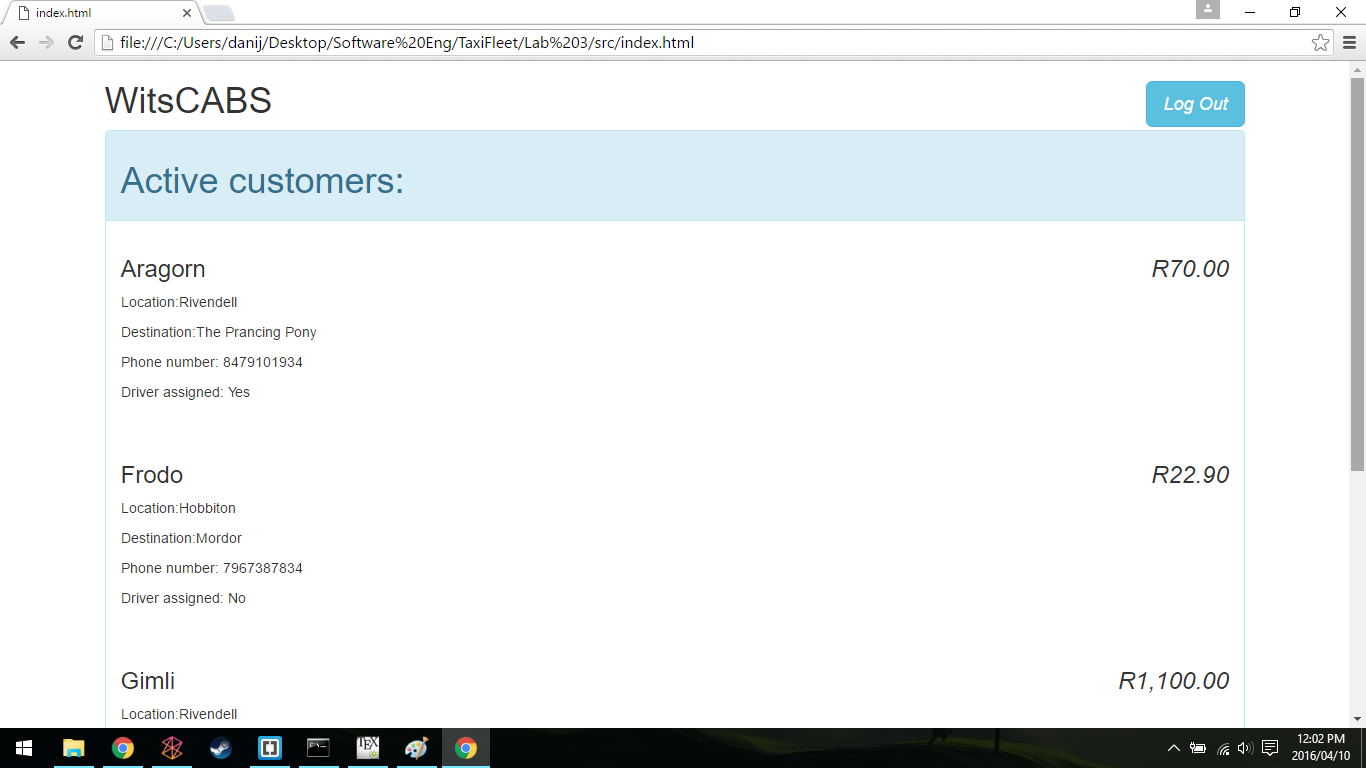
\includegraphics[width=1\textwidth]{DCC active panel.png}
\caption{DCC view with active customers panel.}
\end{figure}

\begin{figure}[ht]
\centering
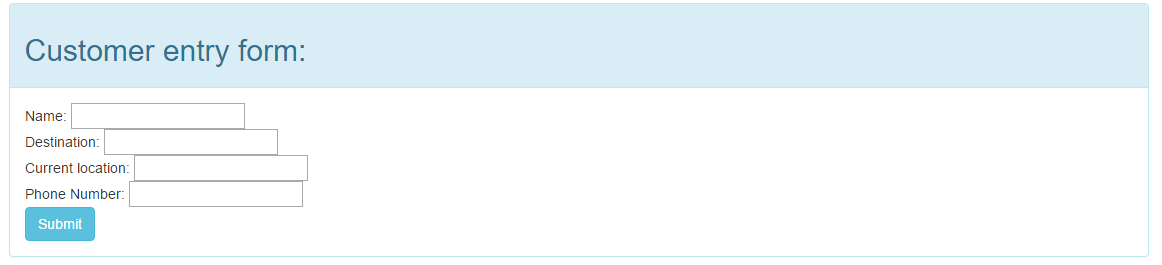
\includegraphics[width=1\textwidth]{new customer form.png}
\caption{DCC view with new customer form.}
\end{figure}

\begin{figure}[ht]
\centering
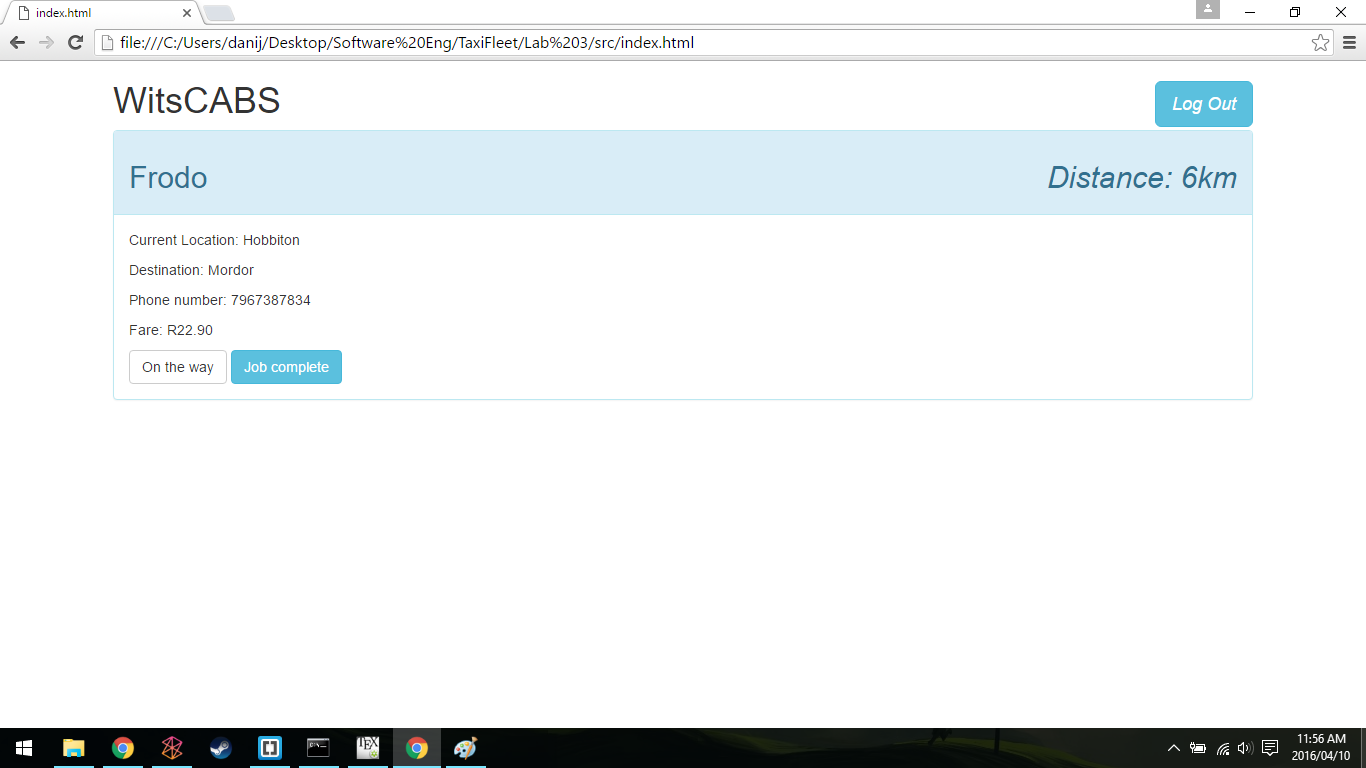
\includegraphics[width=1\textwidth]{driver view.png}
\caption{Driver interface view.}
\end{figure}

\begin{figure}[ht]
\centering
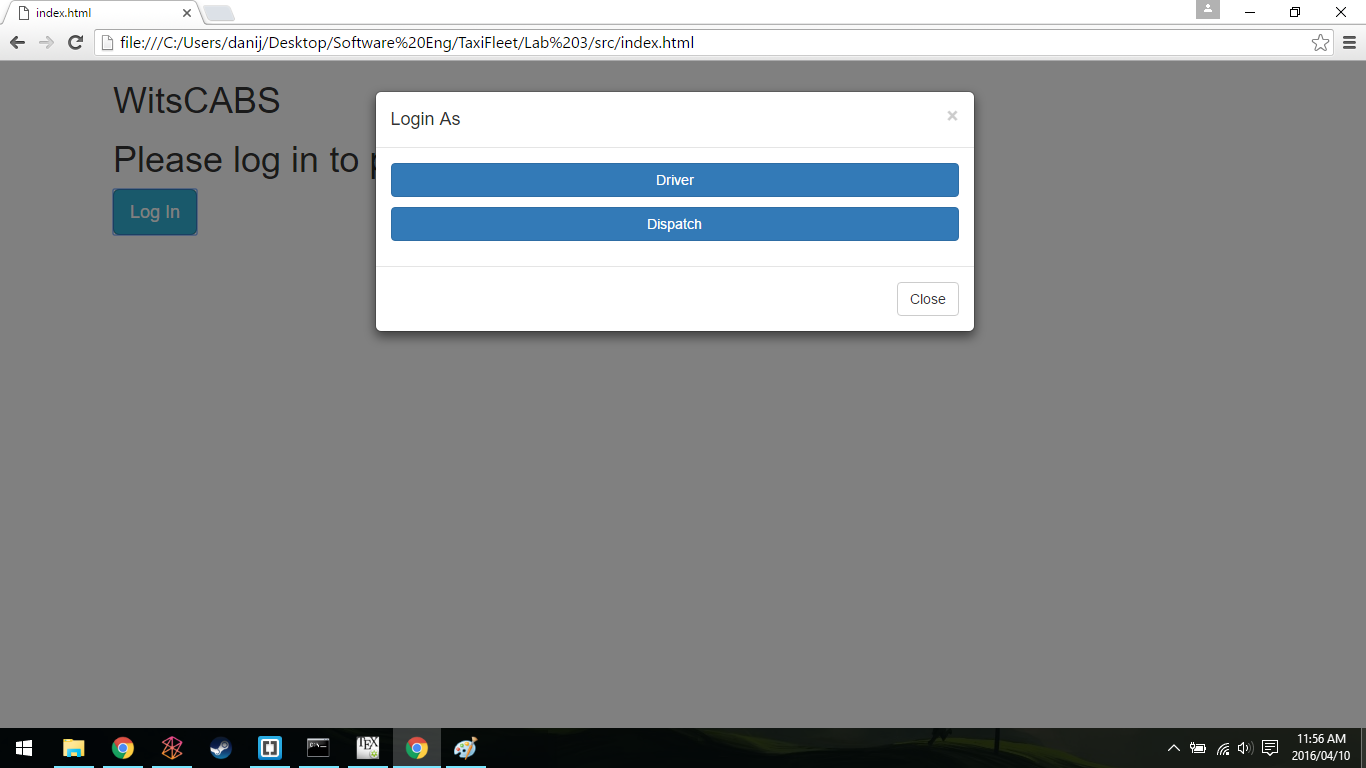
\includegraphics[width=1\textwidth]{login screen and pop up.png}
\caption{Log-in view with pop-up modal.}
\end{figure}


The front-end is implemented using angular.js and Bootstrap3. Included in the HTML file are URL source links for the angular.js library, the Bootstrap stylesheets and a jQuery plugin. This means that the user merely needs to open the HTML file, which will run if the user has internet access. No additional programs need to be installed. For coding, the front-end framework, the text editor Brackets was used. The front-end views for the driver and DCC interfaces were coded by Danielle Winter and Frederick Nieuwoudt.A pair programming method was used for implementing this system. The work breakdown for the prototype implementation is given below:

\begin{itemize}
\item Frederick Nieuwoudt (Scrum Master):
\begin{itemize}
\item Driver interface implementation
\item Login/log-off
\item Commenting DCC code
\item System aesthetics
\item System modifications
\end{itemize}
\item Danielle Winter (project manager):
\begin{itemize}
\item Driver interface commenting
\item Login/log-off commenting
\item DCC interface implementation
\item System aesthetics
\item System modifications
\end{itemize}
\end{itemize}



\subsection{Product Backlog}
\begin{tabular}{|c|l|c|}
\hline 
Interface & Features & Expected Time (Days)\\ 
\hline 
DCC & Active jobs panel & 5\\ 
• & Customer form panel & 5\\ 
• & Implement tabbed view (rather than panels) & 1 \\
• & Automatic address completion using Google Maps API & 5\\

\hline 
Driver & Assigned job panel & 5\\
• & Buttons for "On the way" and "Job complete" & 1\\ 
• & Automatic update of navigation & 5\\
\hline 
General & Log-in page & 5\\ 
• & Log-in authentication & 5\\
• & Create basic interface framework & 1\\
• & Set up AngularJS customer directive & 2\\
• & Review user experience design (aesthetics using CSS) & 5\\
• & Set up google maps API & 5\\
\hline
\end{tabular} 
\subsection{Sprint Planning}
Sprint planning was undertaken to divide tasks in such a way that the most efficient path was taken.\\

In order to achieve this the task back log was represented on a gantt chart in order to visualize the product dependencies and which tasks could happen in parallel. The produced gantt char is available in the figure below.\\

\begin{figure}[ht]
\centering
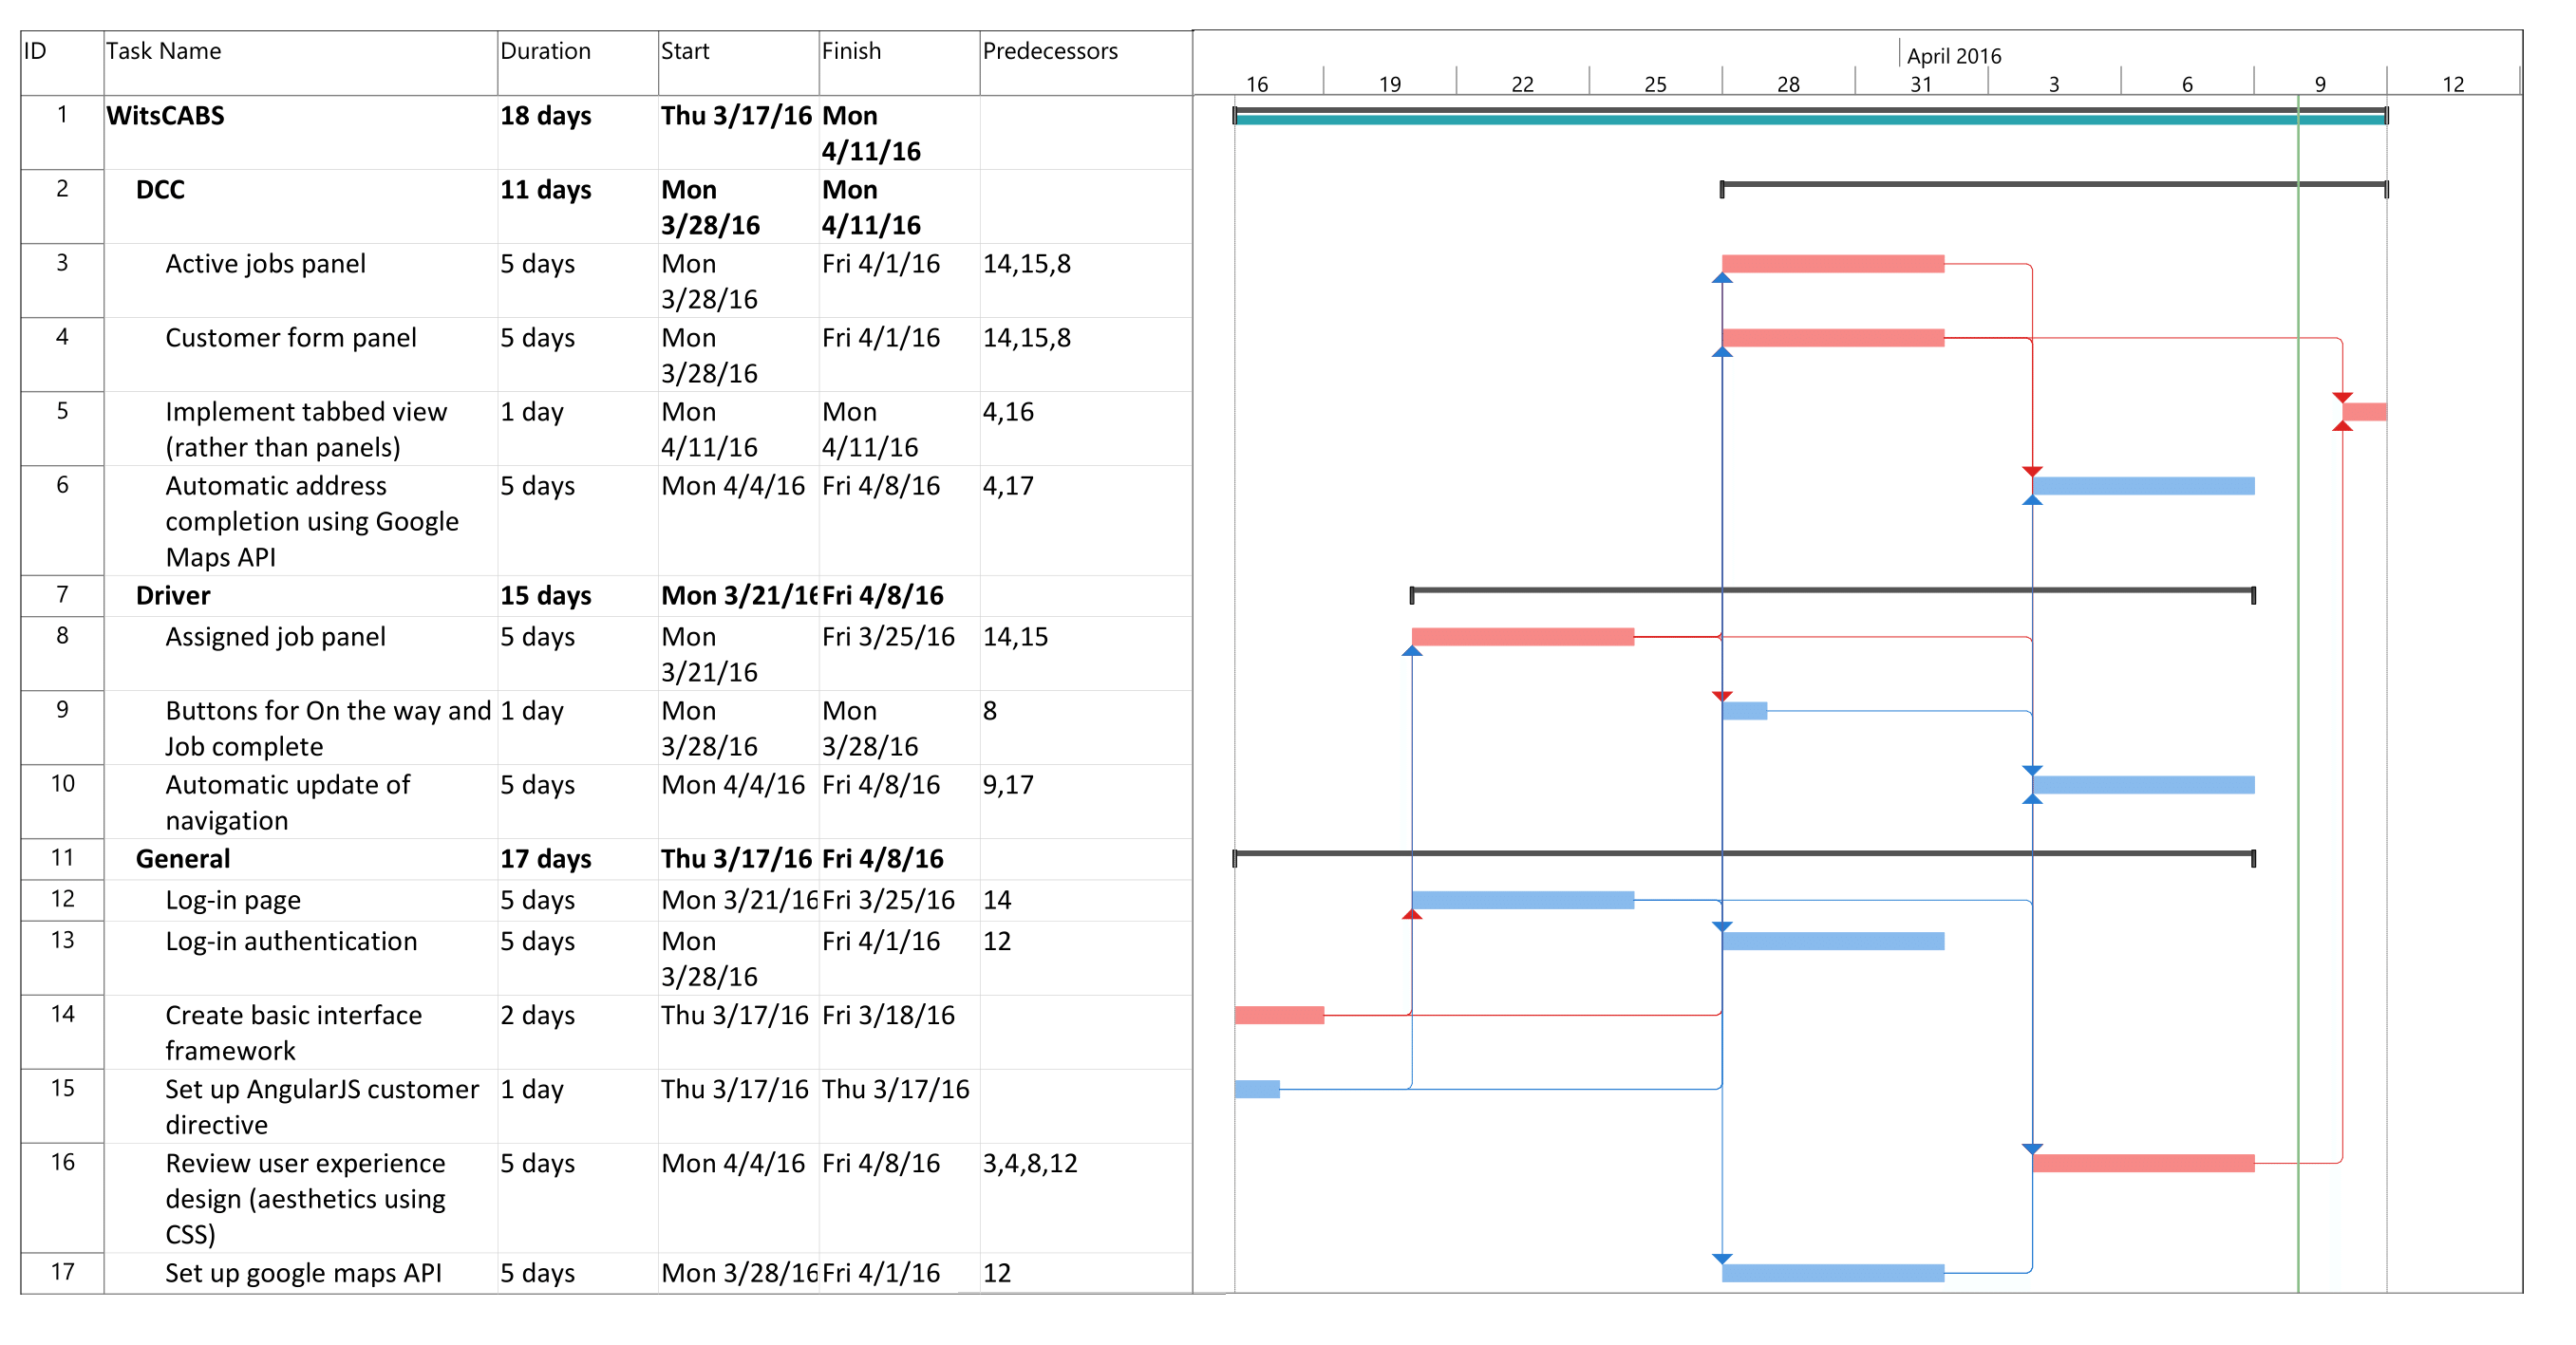
\includegraphics[width=1\textwidth]{gantt.png}
\caption{Gantt chart showing all required tasks and their dependencies.}
\end{figure}
The tasks were divided according to whether they were on the critical path or not. Creating the views for specific users was the most important for the success of the prototype. Tasks such and login authentication and the addition of Google maps functionality were not critical to the creation of a prototype that can visually demonstrate the final product.
\subsection{Sprint Retrospective}
Three sprints were completed to produce the presented front-end prototype. The features implemented in each sprint has been cataloged in the table below.\\

\begin{tabular}{|c|l|c|}
\hline 
Sprint & Features\\ 
\hline 
 1 & Create basic interface framework\\ 
• & Set up AngularJS customer directive\\

\hline 
 2 & Driver assigned job panel\\
• & Create default login page\\
• & Create login modal\\
\hline 
 3 & Add DCC active jobs panel \\ 
 • & Add DCC customer form panel\\
 

\hline
\end{tabular} 





%%%%%%%%%%%%%%%%%%%%%%%%%%%%%%%%%%%%%%%%%%%%%%%%%%%%%%%%%%%%%%%%%%%%%%%%%%%%%%%%%%%%%%%%%%%%%%%%%%%%%%%%%%%%%%%%%%%%%%%%%%%%
\newpage
\section{PART B: BACK-END}
\subsection{SRS}
\subsection{SDS}
\subsection{Prototype Implementation}
\subsection{Product Backlog}

\subsection{Sprint Planning}
\subsection{Sprint Retrospective}


\end{document}